\documentclass[journal=jacsat,manuscript=article]{achemso}

\usepackage{graphicx}
\usepackage{amsmath}

\bibliographystyle{achemso}

\author{Oliver T. Unke}
\affiliation{Department of Chemistry, University of Basel, Klingelbergstrasse 80, CH-4056 Basel, Switzerland.}

\author{Markus Meuwly}
\affiliation{Department of Chemistry, University of Basel, Klingelbergstrasse 80, CH-4056 Basel, Switzerland.}
\email{m.meuwly@unibas.ch}

\date{\today}

\title{}

\begin{document}

\begin{abstract}

\end{abstract}

\clearpage

\section{MS-ARMD}
\label{sec:msarmd}
Following a chemical reaction to determine the reaction pathway and to
predict experimental observables is a key task for computational
methods, since most atomistic aspects can not be determined
experimentally.\cite{brooks.chemrev.1988.msarmd} Using quantum methods
is usually inexpedient for large systems for the simple reason that
the computational requirements are too high. Hence alternative
approaches, like QM/MM\cite{warshel.jmb.1976.msarmd} and reactive
force fields (FF) have been developed. The former, however, can not be
utilized to calculate converged reaction rates, due to the high
computational cost of calculating hundreds, long-time
trajectories. Therefore accurate reactive FF approaches offer the best
means for sampling processes of interest in a statistically convincing
approach.\\

\noindent
Among other methods, such as the work by Warshel
(EVB)\cite{warshel.jacs.1980.msarmd}, Westmoreland
(RMDff)\cite{westmoreland.molsimul.2007.msarmd}, van Duin and Goddard
(ReaxFF)\cite{vanduin.jpca.2001.msarmd}, Meuwly and coworkers
developed multisurface adiabatic reactive molecular dynamics
(MS-ARMD)\cite{MM06cross,rmd08,nagy.jctc.2014.msarmd}. This method,
which aims to achieve quantum method accuracy with, in principle, the
computational cost of conventional FF, couples (at least) two
non-reactive, empirical FFs by means of a time- or energy-independent
switching function $w_i$. MS-ARMD is a widely applicable technique
that can describe several different reaction pathways and conserves
total energy. It was implemented in the widely used CHARMM
program\cite{brooks.jcc.2009.msarmd}.\\

\noindent
In MS-ARMD adiabatic dynamics takes place on the lowest potential
energy surface (PES) $V_{\text{min}}$, as long as the energy of the
higher lying surface(s) is not within a specified, user defined
$\Delta V$ of energy. Surface-crossing is achieved by mixing the PESs
through energy-dependent weights. $\Delta V$ acts as energy damping
parameter that balances the individual weights with respect to the
energy separation (``gap'') between the PESs. Products of Gaussian and
polynomial functions (GAPOs), which depend on the energy difference
between two surfaces ($\Delta V_{ij}$), are introduced for the purpose
of reproducing the energy barrier from electronic structure
calculations. The global, reactive PES is therefore described by

\begin{equation}
  V_{\text{MS-ARMD}}(x) =\sum_{i=1}^n w_i(x)V_i(x) + \sum_{i=1}^{n-1} \sum_{j=i+1}^n [w_i(x)+w_j(x)]  \sum_{k=1}^{n_{ij}} \Delta V_{\text{GAPO},k}^{ij} (x)
  \label{eq:msarmd}
\end{equation}

\noindent
where $w_i(x)$ are normalised weights obtained from raw weights
$w_{i,0}(x)$, calculated by $w_{i,0}(x) = \exp (- (V_i(x) -
V_{\text{min}})/ \Delta V)$, $V_i(x)$ is the energy of state $i$ and
$\Delta V_{\text{GAPO},k}^{ij} (x)$ is the energy of the GAPO between
state $i$ and $j$. Evaluating energies and forces in MS-ARMD scales
linearly with number of low lying surfaces. The time liming factor in
this approach is fitting of a suitably parametrised PES.\\

\begin{figure}
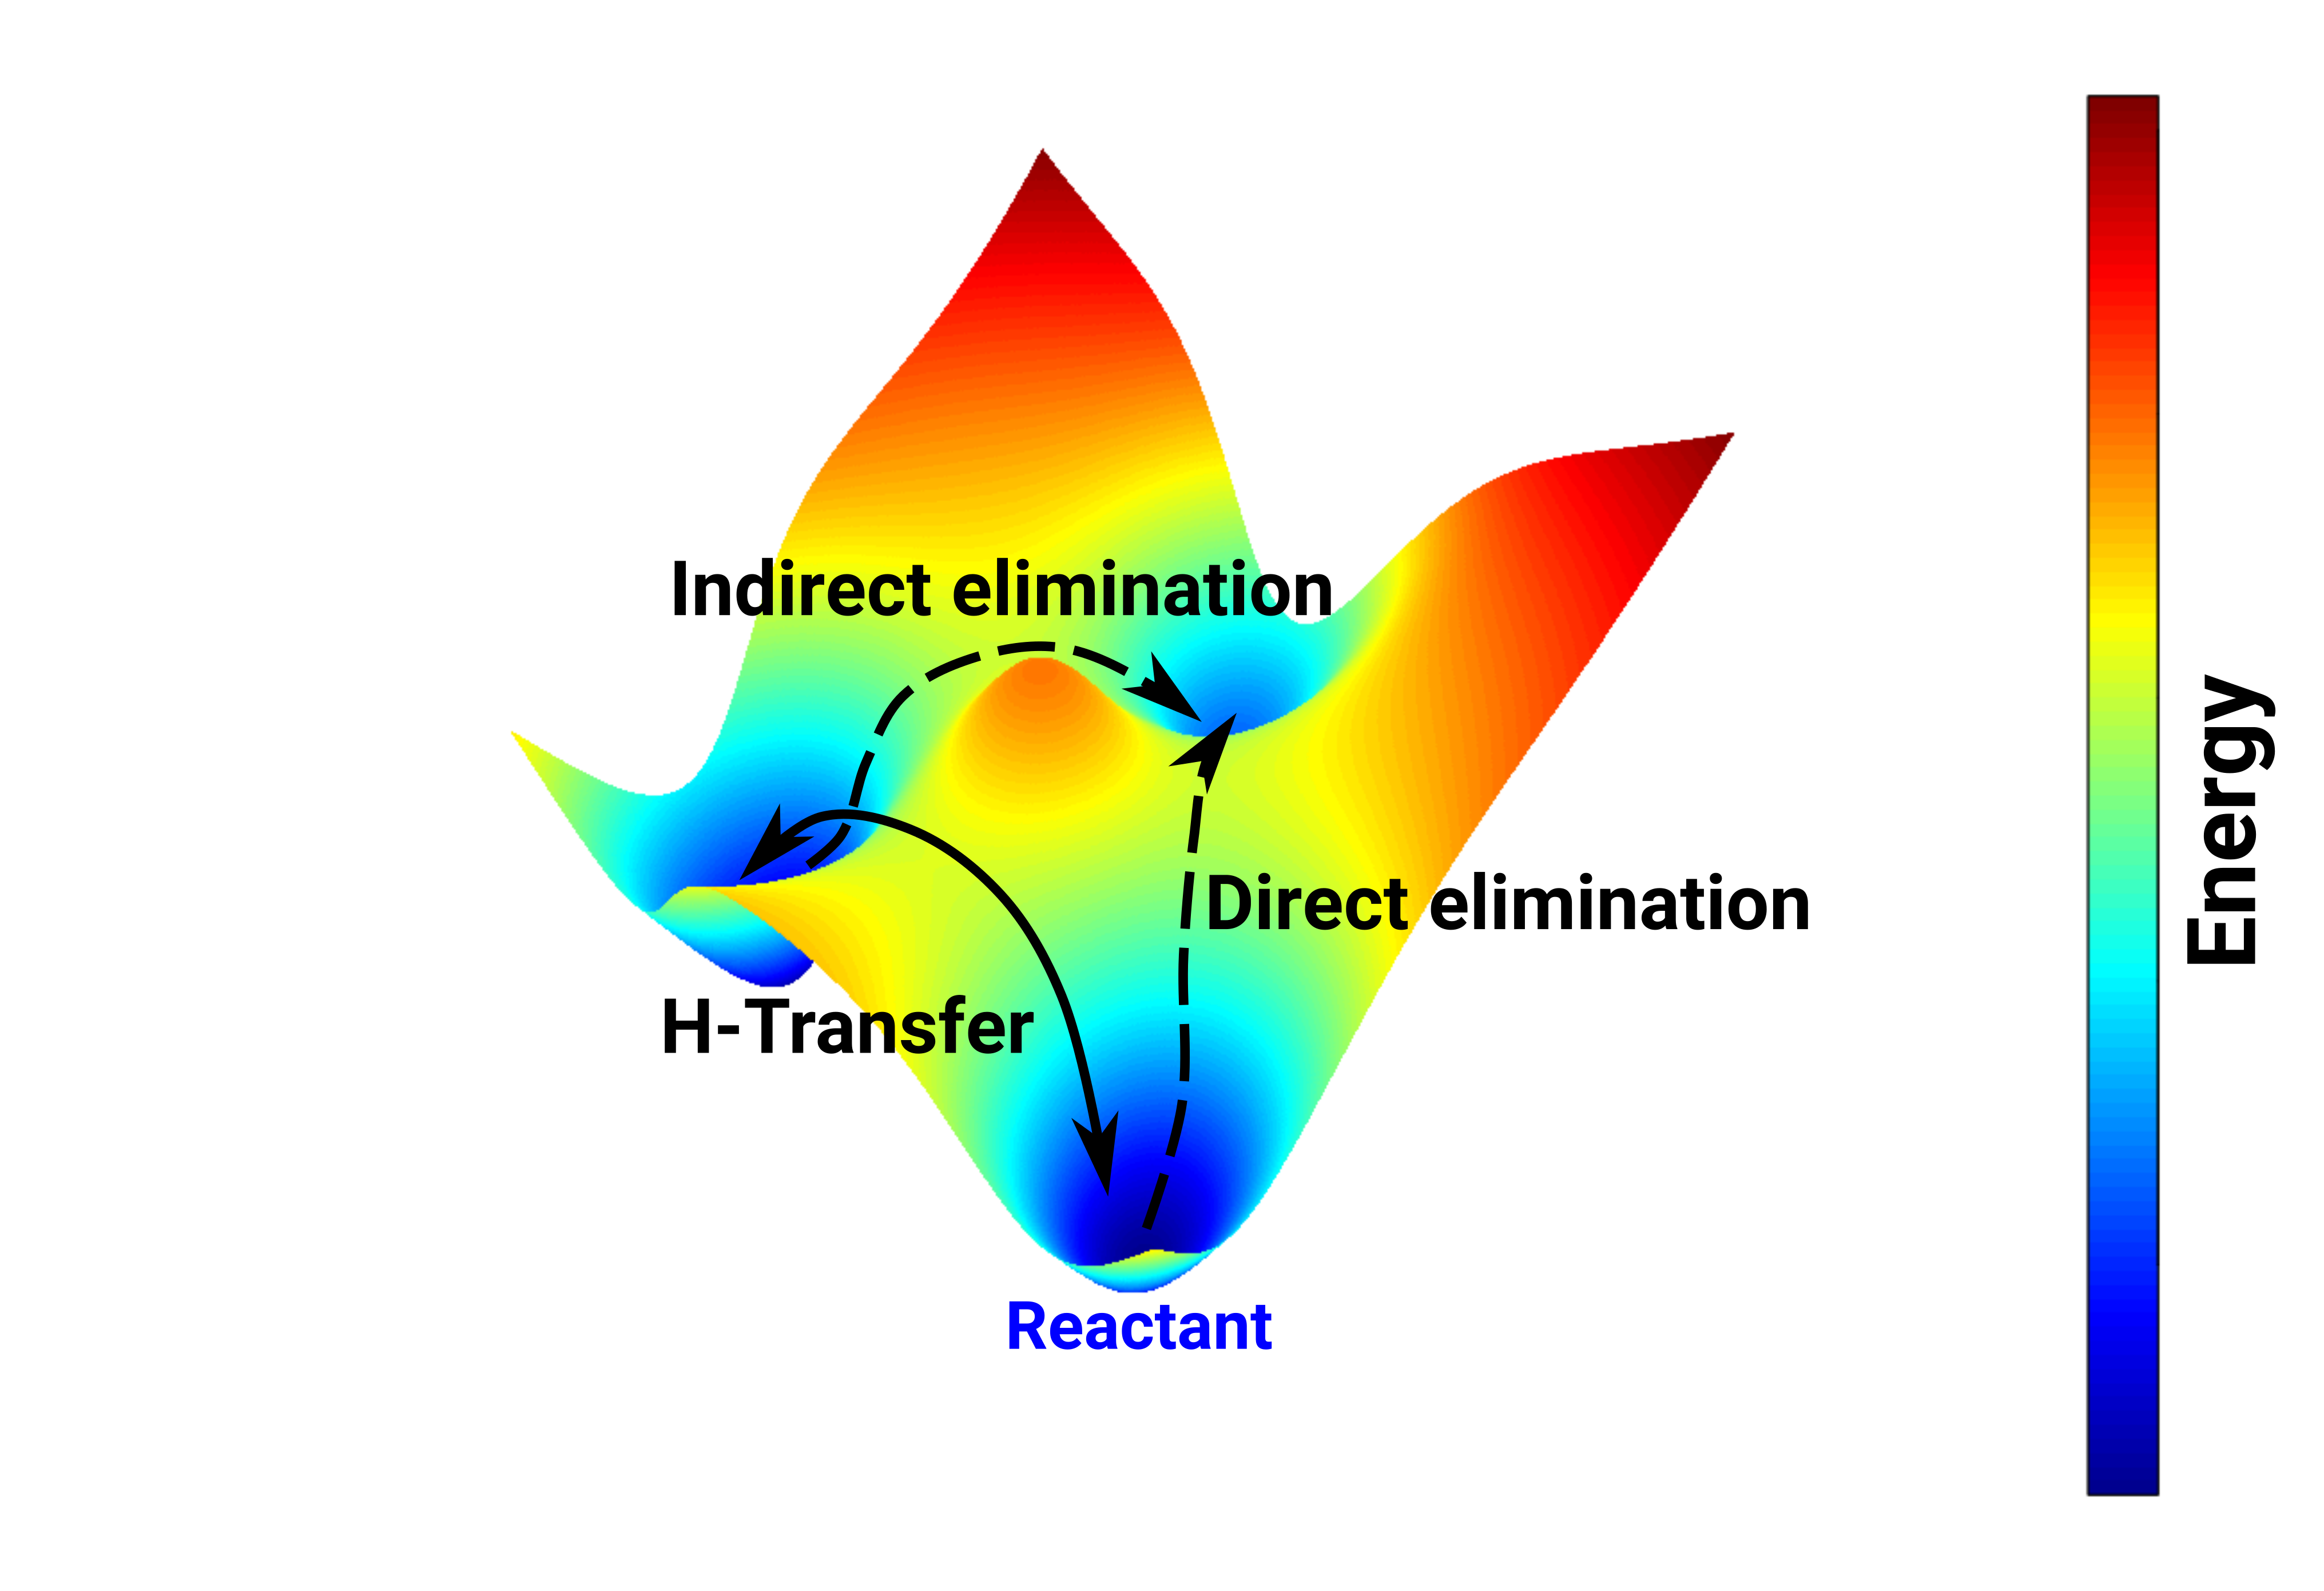
\includegraphics[width=\textwidth]{fig/msarmd-sulphonics.png}
\caption{Simplified schematic representation of the PES of sulphuric
  acid and its derivatives, including minima of the reactant, the
  H-transfer product, and the elimination product.}
	\label{fig:msarmdsulphonic}
\end{figure}


\subsection{Sulfuric Acid}

\noindent
The power of MS-ARMD lies in the calculation of converged reaction
rates because thousands of individual trajectories can be run, which
allows for quantitative characterisation of final state
distributions. This is usually not possible for conventional mixed
quantum mechanics/classical mechanics (QM/MM)/MD or full QM/MD
simulations due to the computational expense in the quantum region. An
example for such an application is the vibrationally induced
photodissociation of sulphuric acid in the gas phase, where the
excitation of a OH stretching vibration lead to photofragmentation
into water and sulphur-trioxide\cite{reyes.pccp.2014.msarmd}. This
reaction has also been investigated using QM/MD simulations at the PM3
level of theory.\cite{Miller:2006}\\

\noindent
After excitation of the local $\nu_9$ normal mode H$_2$SO$_4$ can
follow two different reaction pathways: intramolecular H-transfer and
water elimination. The global PES for modelling the reactions was
parametrised to several thousand MP2/6-311G++(2d,2p) reference
electronic structures, describing the H$_2$SO$_4$, H$_2$O, SO$_3$, and
the van der Waals complex of water and sulphur-trioxide. Due to the
fact that atom indices utilised to define the connectivity within a
molecule a total of 16 states (permutation invariant surfaces) were
used in the calculations (12 describing the chemically equivalent
conformations of H$_2$SO$_4$ and 4 describing the chemically
equivalent conformations of the elimination products). Each state can
undergo six different reactions, four leading to different
conformations of the reactant and two leading to H$_2$O and
SO$_3$. The system was set up by heating the geometry optimised
structure of H$_2$SO$_4$ to 300 K. The leapfrog Verlet algorithm was
used for 40 ps of equilibration and 50 ps of free dynamics. The
excitation of the OH stretching vibration was achieved by scaling the
instantaneous velocities along the normal mode. A Morse potential was
used for describing the excitation energies of the OH stretch.\\

\noindent
Several thousand independent trajectories with a simulation time of 1
ns resulted in 58\%, 77\%, and 80\% of water elimination for the
excitation with $\nu_9$ = 4,5, and 6, respectively. The final state
analysis, which predicts the expected findings of an experimental
investigation. It was found that if H-transfer precedes the water
elimination (called indirect) the excess energy distributes preferably
into vibrational and rotational degrees of freedom. In contrast,
direct water elimination (without prior H-transfer) leads to
redistribution into translational energy. Fitting of a simple kinetic
model to the obtained date enables the determination of relaxation
($\tau_{\text{IVR,i}}$) and decomposition times ($\tau_i$) for
different excitation energies.\\

\subsection{Chlorosulfonic Acid}

\noindent
{\bf Need also refs to Kjaergaard papers here.} Due to experimental
difficulties in the investigation of the overtone-induced
photodissociation of H$_2$SO$_4$ the mechanism was further
investigated using HSO$_3$Cl as a
proxy\cite{reyesbrickel.pccp.2016.msarmd}. The system was set similar
to the calculations of H$_2$SO$_4$, with the difference of the total
time of free dynamics (increased 250 ns), maximum simulation time
(increased to 2.5 ns), and the number of independent trajectories
(decreased to 5000).\\

\noindent
Comparing the photofragmentation of HSO$_3$Cl to the one of
H$_2$SO$_4$ a substantial difference in the percentage of reactive
trajectories leading to elimination can be observed. For HSO$_3$Cl the
yield of HCl elimination after 1 ns of simulation is
increased. Furthermore the ratio between direct and indirect
switches. For sulphuric acid the rate of intramolecular H-transfer is
constant and secondary in comparison to direct water
elimination. These differences can be explained by the transformation
of symmetry and the more rapid elimination in H$_2$SO$_4$
,respectively. The vibrational energy distribution of HCl, which is
experimentally the most amenable observable, reveals a slight bimodal
$j$-distribution for higher excitation degrees. This can be explained
by differences in the redistribution of energy. For indirect
elimination the excess energy goes more into other modes as for direct
elimination. The latter therefore peaks at lower $j$ values. For the
simulations of HSO$_3$Cl it was further shown, by running simulations
on an ensemble generated by Monte Carlo sampling, that the conclusions
are reliable and independent of the choice of initial conditions.
 

\section{N$_2^+$ + Ar}
\label{sec:n2plusar}
The collision of N$_2^+$ ions with Ar atoms is a prototypical system
to study ion-atom collisions and charge transfer reactions. It might
also be an example of a system were non-adiabatic effects are
important in order to understand the underlying dynamics. Previous
experiments by Schlemmer \textit{et
  al.}\cite{schlemmer.ijms.1999.n2plusargon} on this system have
uncovered an unusual behaviour regarding the rotational relaxation of
N$_2^+$ ions.  Since the (N$_2^+$-Ar) complex has a large binding
energy of 1.109 eV\cite{mahnert.jcp.1995.n2plusargon}, collisions at
low temperatures should proceed via a long-lived bound state. Since
this usually leads to statistical mixing of all accessible product
channels, a quick redistribution of rotational states can be
expected. However, Schlemmer \textit{et al.} found a very low rate
coefficient of $k_J$(90 K) $= (1.4\pm 0.4) \cdot 10^{-11}$
cm$^3$s$^{-1}$ for rotational relaxation, which implies that the
contrary is true. Assuming that collisions occur at the Langevin rate
$k_L = 7.4\cdot10^{-10}$ cm$^3$s$^{-1}$, this implies that the
rotational state of N$_2^+$ ions is conserved for about 49 out of 50
collisions with Ar atoms (according to the Langevin model, a collision
complex is formed if the collision energy is sufficient to overcome
the rotational barrier).\cite{schlemmer.ijms.1999.n2plusargon}\\

\noindent
Schlemmer \textit{et al.} proposed that this unexpected result could
either be explained as the consequence of some hidden constants of
motion leading to approximate selection rules, or by the presence of
additional barriers in the (N$_2^+$-Ar) potential energy surface
(PES). They remark that ``detailed \textit{ab initio} calculations and
quantum mechanical treatment of the collision dynamics at meV energies
are required to conclusively answer the
question".\cite{schlemmer.ijms.1999.n2plusargon}\\

\noindent
Meuwly and
coworkers\cite{unke.jcp.2016.n2plusargon,denisalpizar.2017.n2plusargon}
constructed a state of the art (N$_2^+$-Ar) PES based on \textit{ab
  initio} energies computed at the UCCSD(T)-F12a/aug-cc-vtz level of
theory using reproducing kernel Hilbert space (RKHS)
theory.\cite{hollebeek.annrevphychem.1999.rkhs,unke.2017.rkhstoolkit}
The RKHS method has the appealing quality that it exactly reproduces
the given data, therefore allowing energy evaluations at practically
\textit{ab initio} quality.\cite{unke.jcp.2016.n2plusargon} In order
to assess the importance of multireference effects, additional
calculations at the CASSCF/MRCI+Q level of theory were performed and
it was concluded that UCCSD(T)-F12a/aug-cc-vtz is a sufficiently high
level of theory.\cite{denisalpizar.2017.n2plusargon} Quantum
close-coupling calculations\cite{denisalpizar.2017.n2plusargon} as
well as quasi-classical trajectory (QCT)
calculations\cite{unke.jcp.2016.n2plusargon,denisalpizar.2017.n2plusargon}
were performed on the RKHS-PES using conditions similar to those in
the experiment by Schlemmer \textit{et
  al.}\cite{schlemmer.ijms.1999.n2plusargon} The rate coefficients for
rotational relaxation obtained by the quantum and QCT calculations
agree favourably and range between $5.34 \cdot 10^{-10}$
cm$^3$s$^{-1}$ and $6.96 \cdot 10^{-10}$
cm$^3$s$^{-1}$.\cite{denisalpizar.2017.n2plusargon} These rates are in
line with the expected quick redistribution of rotational states and
suggest that more than 70\% of collisions lead to a change of the
rotational quantum state.\\

\noindent
Due to the high quality of the PES and the agreement of
quasi-classical and quantum results, it is unlikely that the
discrepancy to the experimentally observed rate is due to deficiencies
of the applied computational methods. However, it is possible that the
Born-Oppenheimer approximation is not valid for the (N$_2^+$-Ar)
complex and non-adiabatic effects are important in the dynamics. This
assumption is supported by the observation that lowest excited
electronic state of (N$_2^+$-Ar) is only energetically separated by
about 700 cm$^-1$ from the ground state in the long range part of the
N$_2^+$ + Ar interaction (Fig. \ref{fig:n2arlevels}). In fact, the
separation of the electronic states is a function of the vibrational
motion that the N$_2^+$ undergoes and therefore suggests that a
coupling between nuclear and electronic degrees of freedom might
exist.\cite{denisalpizar.2017.n2plusargon}

\begin{figure}
\includegraphics[scale=0.3]{fig/n2arlevels.png}
\caption{Interaction energy at the inner turning point ($r = 1.072$
  \AA\/) of the $v = 0$ vibration for the three lowest electronic
  states of (N$_2^+$-Ar) (the angle between $r$ and $R$ is
  $168^{\circ}$). The curves were computed at the MRCI+Q/avtz level of
  theory in the $^2$A$'$ symmetry. Note that the separation between
  ground state and first excited state is only about $700$ cm$^{-1}$
  at around $R=4.5$\AA\/.}
\label{fig:n2arlevels}
\end{figure}
    
\section*{Acknowledgments}
The NCCR MUST (to MM) and the University of Basel are acknowledged.


\bibliography{../literature}

\end{document}
